%%% INTRODUCTION %%%

3D printing technologies provide the ability to produce new parts quickly, allowing faster and cheaper design iterations. However current FDM (Fused Deposition Modeling) printers produce relatively weak parts due to the plastics used and the low inter-layer adhesion area in thin features. These considerations limit FDM 3D printing to prototpying applications. Stronger parts could be created in FDM printers by using new materials and print methods. CFRP (Carbon fiber reinforced polymers) are a good candidate because are already widely used in industry load-bearing applications and are laid up in a similar fashion to how 3D FDM printing works. Some printers can even print continous carbon fibers, but not in contoured layered optimized for part strength \cite{markforged}. Since the behavior of CFRPs under loading depends largely on the fiber orientation in and between fiber layers, a CFRP FDM printer would need the ability to lay carbon fiber in any orientation, to create the optimal fiber angles for any load case as well as to optimize inter-layer adhesion area. 

The main goal of the project for this academic year was to set up a 6-degree-of freedom robot arm as a CFRP 3D printer, develop a continuous-fiber CFRP filament, print test specimens, and test the specimens for desirable mechanical properties with respect to FEA-predicted results and current 3D printed parts. One specimen geometry was selected for printer development and is shown in Figure~\ref{fig:intro-layers-geometry-loads}. Given the applied loads to the bridge specimen, curved layers CFRPs should easily react bending induced in the arch while a planer part would prematurely delaminate due to limited adhesion area and weak plastic material. 

\begin{figure}[t]
\centering
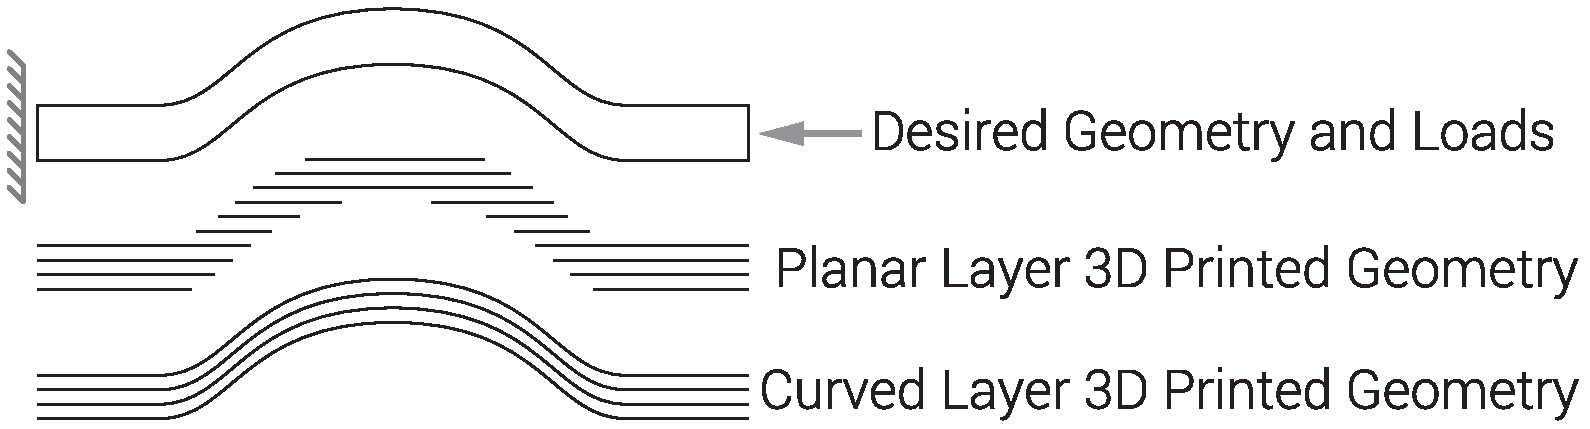
\includegraphics[width=0.8\linewidth]{./figures/intro-layers-geometry-loads}
\caption{Printing layer geometry and applied loads}
\label{fig:intro-layers-geometry-loads}
\end{figure}